\section{Versuchsaufbau/-durchführung}

\subsection{Versuchsaufbau}
Der grundlegende Aufbau ist in der Abbildung \ref{fig: aufbau} abgebildet.
\begin{figure}[h]
  \centering
  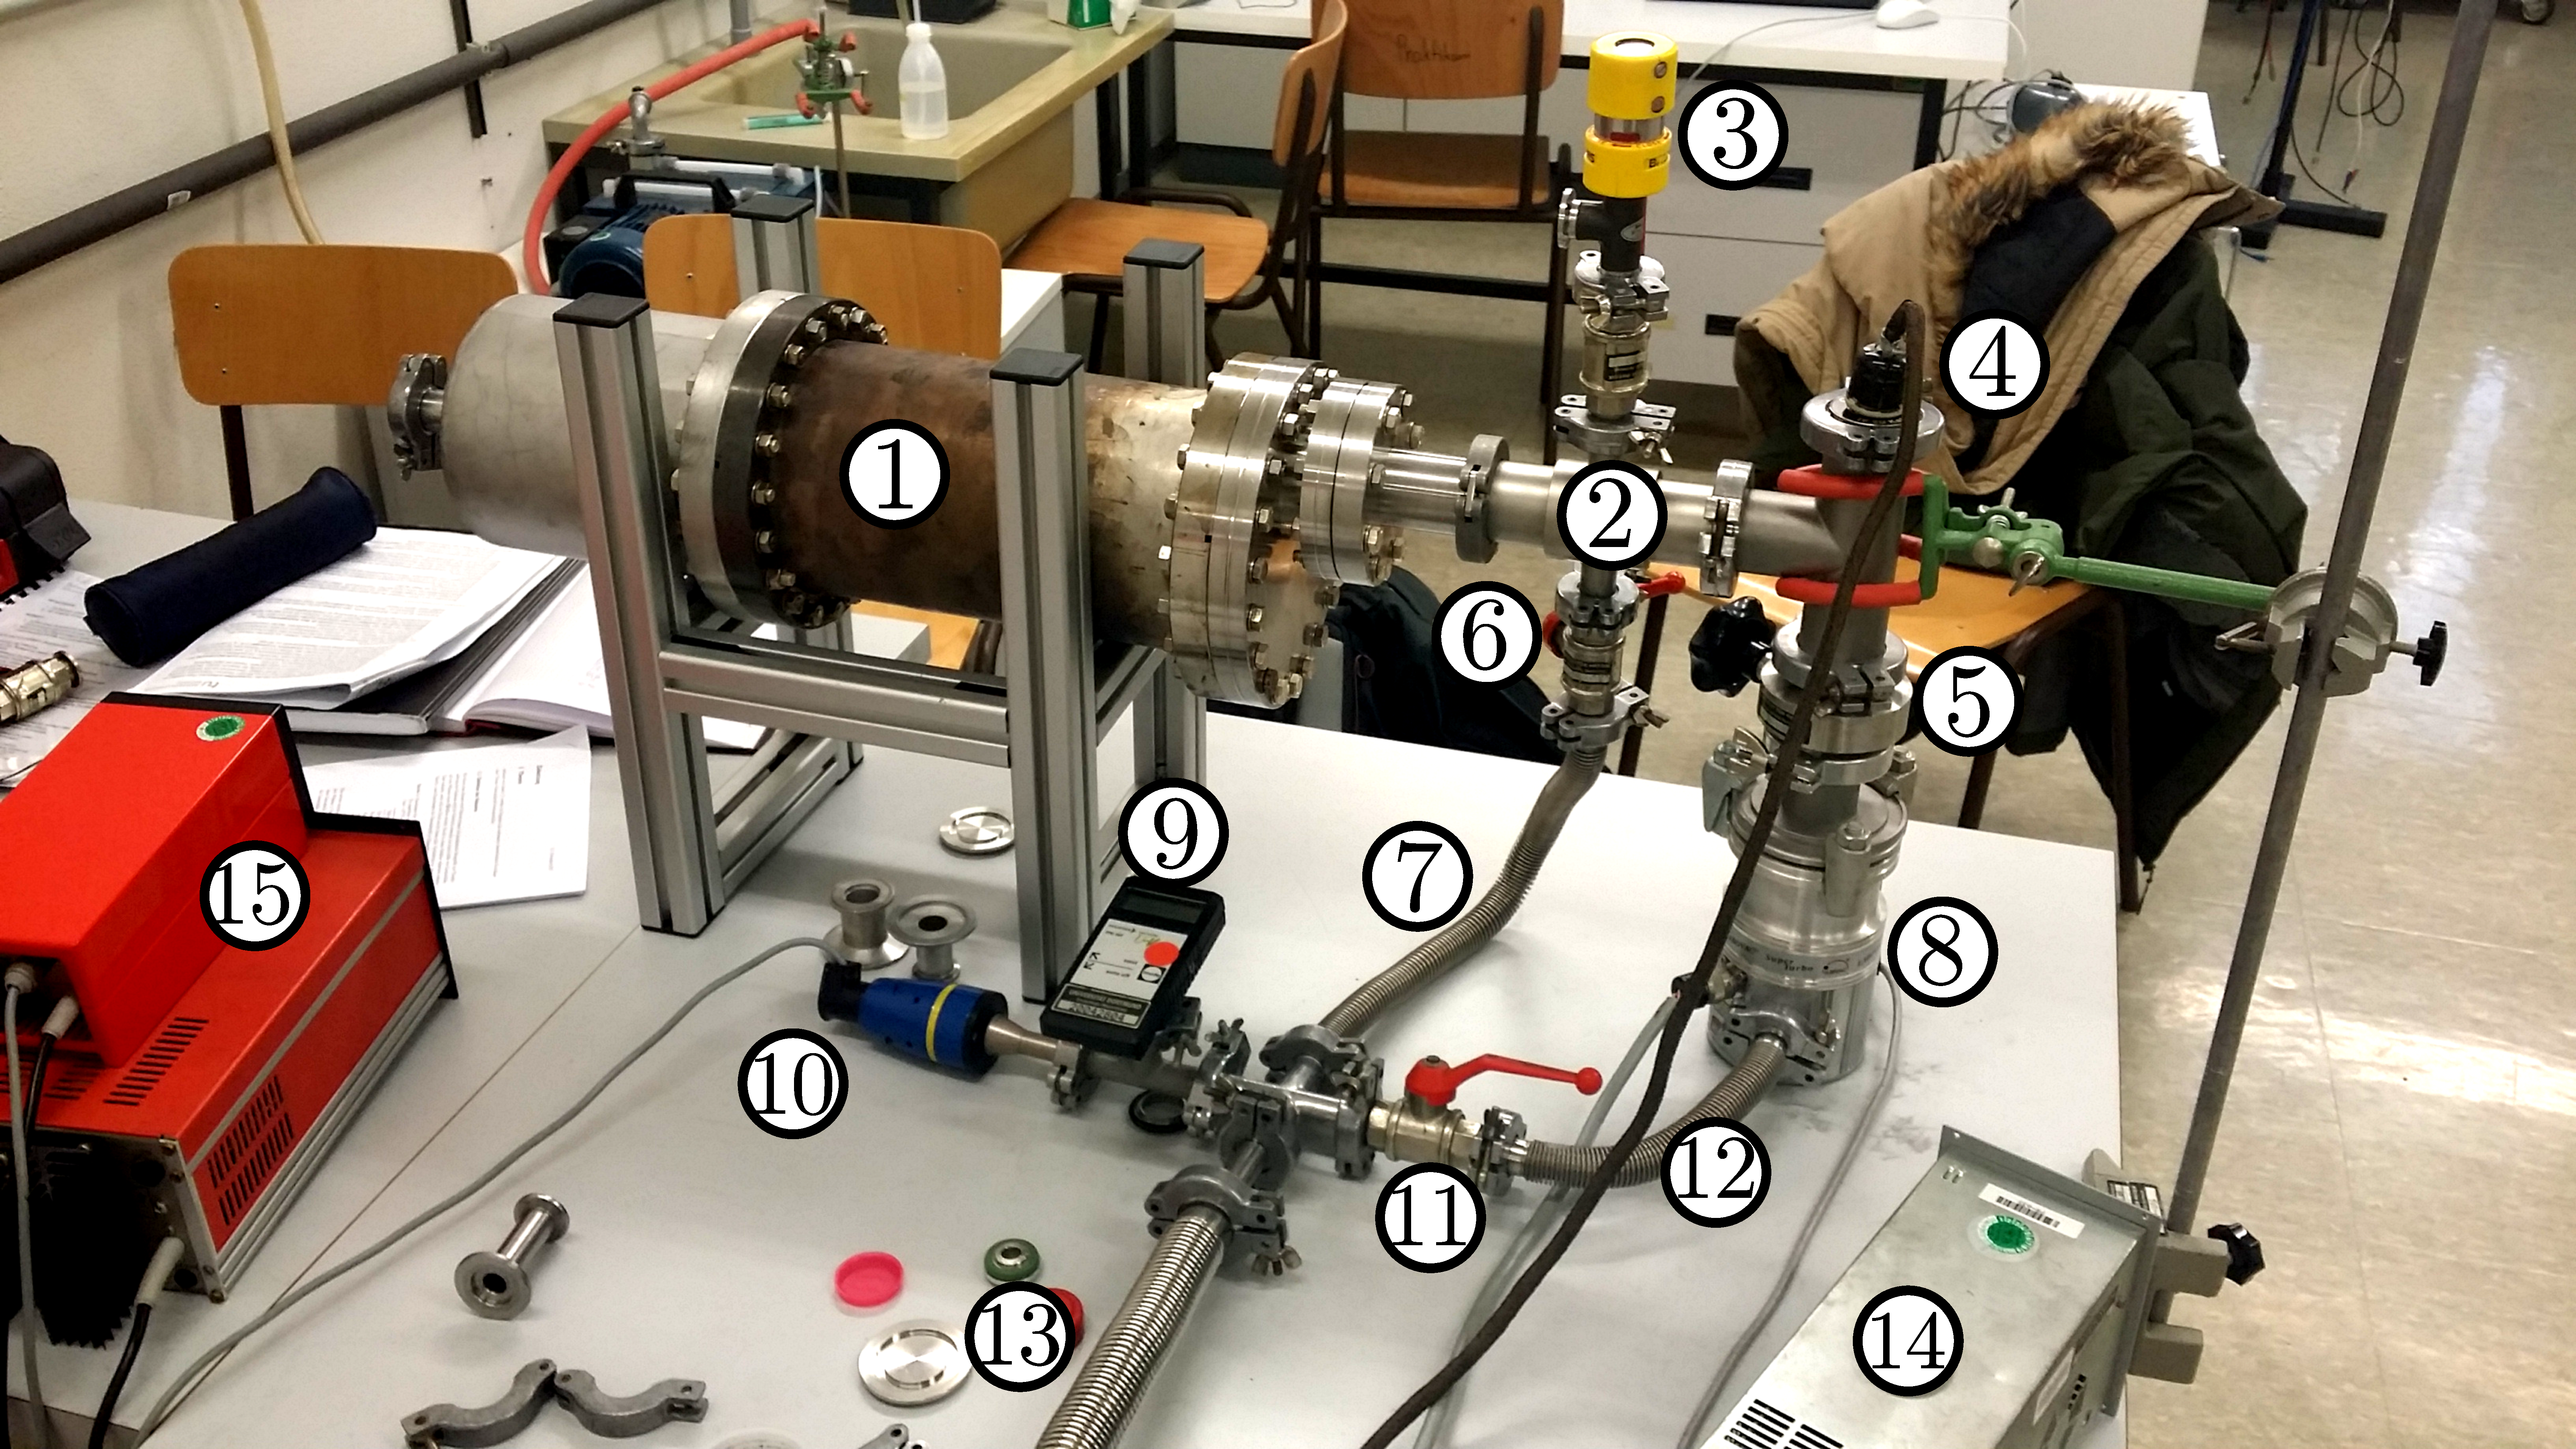
\includegraphics[width=0.6\textwidth]{./pics/aufbau.png}
  \caption{Grundlegender Aufbau eines Rastertunnelmikroskops \cite{rtm}.}
  \label{fig: aufbau}
\end{figure}
In der Abbildung ist die Spitzenhalterung zu sehen und
der Carrier mit Probe. Die Apperatur wird mittels Computersoftware gesteuert.
Die Spitze wird mit Hilfe von Piezokeramiken filigran bewegt, somit
ist ein präzises Abrastern der Probe möglich.

Beim Abfahren der Probe, gibt es zwei Methoden die Struktur der Probe zu erfassen.
Zum einen ist es möglich den Abstand zwischen Probe und Spitze konstant zu lassen
und die Veränderung des Tunnelstroms zu messen.
Jedoch bietet diese Methode die Gefahr, dass die Spitze die Probe rammt und so unbrauchbar wird
Umgekehrt ist es möglich den Tunnelstrom konstant zu lassen und den Abstand zu variieren.
Die in der Theorie angesprochende Näherung, dass die Auslenkung des Piezokrostalls linear
mit dem anliegenden Feld geht ist in der Realität kaum zu beobachten. Deshalb wird eine
geeignete Software benötigt, die eine genaue Ansteuerung des Piezokristall ermöglicht.
Die im Versuch verwendete Software bietet drei verstellbare Parameter P,S \textbf{Hier noch weiter schreiben}.
% Messverfahren P,S siehe das Skript von der Uni Frankfurt


\subsection{Versuchsdurchführung}

% Spitze ziehen, Draht
% Reinigung, Einsetzen, spitzen Strom einschalten, manuelles heranfahren (Spiegelbild), automatischs Heranfahren
% Statuslämpchen
% Upward Downward
